\documentclass[../main.tex]{subfiles}
\begin{document}
\chapter{Basic Calculus}
\section{Introduction}
Differential equations appear in almost all branches of science and applied mathematics.
\begin{example}[Newton's Second Law]
  \[
    \underbrace{m}_{\text{Mass}} \ddot{x} = \underbrace{F(x, t)}_{\text{Force}}
  \]
  This equation relates the rate of change of position $x$, the \textit{dependant variable}, with time $t$, the \textit{independent variable}.
\end{example}
\section{Differentiation}
\begin{definition}[Derivative]
  The \textit{derivative} of a function $f(x)$ with respect to its argument $x$ is defined as:
  \[
    \deriv{f}{x} = \lim_{h \to 0} \frac{f(x + h) - f(x)}{h}
  \]
\end{definition}
\begin{remark}[Notation]
  We sometimes also use the notation $f'(x)$ or $\dot{f}(x)$ (The dot notation is usually used when $f$ is a function  of time).
\end{remark}
The derivative of a function allows us to determine the gradient of a function at a particular point.
% Maybe add plot?
\begin{definition}[Informal Definition of a Limit]
  Informally, if $\lim_{x \to x_0} f(x) = A$ then $f(x)$ can be made arbitrarily close to $A$ by making $x$ sufficiently close to $x_0$.
  (Note that we don't require that $f(x_0) = A$).
  This is explored further in Analysis I.
\end{definition}
\begin{remark}[Note]
  For the derivative to exist we require both the left and right-handed limits to exist and be equal.
  \[
    \lim_{h \to 0^-} \text{ and } \lim_{h \to 0^+} \text{ exist and are equal}
  \]
\end{remark}
\begin{example}
  Consider $f(x) = |x|$ so
  \[
    \at{\deriv{f}{x}}{0} = \lim_{h \to 0} \frac{|h|}{h}
  \]
  But note that the left and right-handed limits are different ($-1$ and $1$) so $f$ is \textbf{not} differentiable at $x = 0$ but is everywhere else.
\end{example}
We can define higher order derivatives for sufficiently smooth functions:
\[
  \deriv{}{x}\left(\deriv{f}{x}\right) = \deriv[2]{f}{x} = f''(x) = \ddot{f}(x)
\]
\begin{remark}[Notation]
  For the $n$th derivative we use the notation:
  \[
    \deriv[n]{f}{x} = f^{(n)}(x) 
  \]
\end{remark}
\subsection{Order Parameters}
Order parameters allow us to compare the behaviour of functions close to a limiting point, usually denoted $x_0$.
\begin{definition}[Big-$O$ Notation]
  \begin{proofcases}
    \begin{case}{$x_0$ finite}
      $f(x)$ is $O(g(x))$ as $x \to x_0$ if $\exists \delta > 0 \text{ and } M > 0$ such that $\forall x$ with $0 < |x - x_0| < \delta$, then $|f(x)| \leq M |g(x)|$.
    \end{case}
    \begin{case}{$x_0$ infinite}
      $f(x)$ is $O(g(x))$ as $x \to \infty$ if $\exists x_1 \text{ and } M > 0 \text{ such that } \forall x > x_1$, then $|f(x)| \leq M|g(x)|$.
    \end{case}
  \end{proofcases}
\end{definition}
From the definition it follows that if $f(x)$ is $O(g(x))$ then $f(x)/g(x)$ is bounded by $M$ as $x \to x_0$.
\begin{remark}[Notation]
This is often written $f(x) = O(g(x))$ although note that the use of the equals sign is an abuse of notation.
This is because $O(g(x))$ is a \textit{class} of functions but in practice using equals is simply more convenient.
\end{remark}
\begin{example}
  As $x \to 0$, $x^2 = O(x)$ but $x \neq O(x^2)$.
\end{example}
% Plot with x^2 x sqrt(x)
\begin{example}
  $\sin 2x = O(x)$ as $x \to 0$ since $|\sin 2x| \leq 2|x|\;\forall x$.
\end{example}
\begin{example}
  $f(x) = 2x^3 - 4x + 12 = O(x^3)$ as $x \to \infty$ since $\forall x > 1$
  \begin{align*}
    |2x^3 - 4x + 12| &\leq 2|x^3| + |-4x| + 12 \\
                     &\leq 6|x^3| + 4|x^3| + 12|x^3| \\
                     &\leq 22|x^3|
  \end{align*}
  So the definition is satisfied with $x_0 = 1 \text{ and } M = 22$.
\end{example}
\begin{definition}[Little-$o$ Notation]
  $f(x) = o(g(x))$ as $x \to x_0$ if \textbf{for every} $\varepsilon > 0, \exists \delta > 0 \text{ such that } \forall x \text{ with } 0 < |x - x_0| < \delta$ ($x$ sufficiently close to $x_0$) then $|f(x)| \leq \varepsilon |g(x)|$.

  If $g \neq 0$ is in the vicinity of $x_0$ but not necessarily at $x_0$ then an equivalent statement is that:
  \[
    \lim_{x \to x_0} \frac{f(x)}{g(x)} = 0
  \]
\end{definition}
\begin{remark}[Notation]
  Often written as $f(x) = o(g(x))$ or $\underline{o}(g(x))$ when handwritten to differentiate it from big O.
\end{remark}

$f(x) = o(g(x))$ loosely means that $f(x)$ is \textbf{much smaller} than $g(x)$ as $x \to x_0$. 
\begin{example}
 $x^2 = o(x)$ as $x \to 0$ as $\lim_{x \to 0} x^2/x = 0$
\end{example}
\begin{example}
  $\sqrt{x} = o(x)$ as $x \to \infty$ as $\lim_{x \to \infty} \sqrt{x}/x = 0$
\end{example}
\begin{remark}[Notes]
  \begin{itemize}
    \item $f(x) = o(g(x))$ is a stronger statement that $f(x) = O(g(x))$. 
      This is because little-o means that we are bounded by any multiple whereas big-O means were are bounded by a given multiple.

      So $f(x) = o(g(x)) \implies f(x) = O(g(x))$ but $f(x) = O(g(x)) \centernot\implies f(x) = o(g(x))$

      E.g. $f(x) = 2x = O(x)$ as $x \to 0$ but $f(x) \neq o(x)$ because $\lim_{x \to 0} 2x/x = 2$.
    \item Constants don't matter. If $f(x) = O(g(x))$ then $af(x) = O(g(x))$ and $f(x) = O(ag(x))$ for any non-zero constant $a$.
  \end{itemize} 
\end{remark}
Order parameters are useful to classify remainder terms before taking limits.
\begin{proposition}
  \[
    f(x_0 + h) = f(x_0) + hf'(x_0) + o(h) \text{ as } h\to0
    \label{derivLittle}
  \]
\end{proposition}
\begin{proof}
  Suppose that we have a remainder/error term $\epsilon(h)$ before taking the limit in a derivative:
  \begin{align*}
    f(x_0 + h) - f(x_0) &= hf'(x_0) + \epsilon(h) \\
    \lim_{h \to 0} \left[\frac{f(x_0 + h) - f(x_0)}{h}\right] &= f'(x_0) + \lim_{h \to 0} \frac{\epsilon(h)}{h}
  \end{align*}
  From the definition of $f'(x)$ the final limit term vanishes so we have $\lim_{h \to 0} \epsilon(h)/h = 0$ and so $\epsilon(h) = o(h)$ as $h\to0$.
  This means that the error term is of order $o(h)$ so we can write:
  \[
    f(x_0 + h) = f(x_0) + hf'(x_0) + o(h) \text{ as } h\to0
  \]
\end{proof}
\subsection{Rules for Differentiation}
We can introduce some rules of differentiation to make it easier to differentiate composite functions.
\begin{theorem}[Chain Rule]
 If $f(x) = F(g(x))$, then:
 \[
   \deriv{f}{x} = F'(g(x))\deriv{g}{x} = \at{\deriv{F}{g}}{g(x)} \at{\deriv{g}{x}}{x}
 \]
\end{theorem}
\begin{proof}
  \begin{align*}
    \deriv{f}{x} &= \lim_{h \to 0} \frac{1}{h} [F(g(x + h)) - F(g(x))] \\
                 &= \lim_{h \to 0} \frac{1}{h} [F(g(x) + hg'(x) + o(h)) - F(g(x))] \\
                 &= \lim_{h \to 0} \frac{1}{h} [\cancel{F(g(x))} + (hg'(x) + o(h))F'(g(x)) + o(hg'(x) + o(h)) - \cancel{F(g(x))}] \\
                 &= \lim_{h \to 0} \frac{1}{h} [hF'(g(x))g'(x) + o(h)F'(g(x)) + o(hg'(x) + o(h))]
  \end{align*}
  For a given $x$, $F'(g(x))$ is constant so $o(h)F'(g(x)) = o(h)$ and similarly $o(hg'(x) + o(h)) = o(h)$. So:
  \begin{align*}
    \deriv{f}{x} &= F'(g(x))g'(x) + \lim_{h \to 0} \frac{o(h)}{h} \\
                 &= F'(g(x))g'(x)
  \end{align*}
\end{proof}
\begin{example}
  $\deriv{}{x} \sin(x^2 - x + 2) = \cos(x^2 - x + 2) \cdot (2x - 1)$
\end{example}
\begin{theorem}[Product Rule]
  If $f(x) = u(x)v(x)$, then:
  \[
    \deriv{f}{x} = v \deriv{u}{x} + u \deriv{v}{x}
\]
\end{theorem}
If we replace $v \mapsto v^{-1}$ and also apply the chain rule then we get the quotient rule:
\[
  \deriv{}{x}\left(\frac{u}{v}\right) = \frac{vu' - uv'}{v^2}
\]
We can also generalise the product rule to the $n$-th derivative using Leibniz's rule:
\begin{theorem}[Leibniz's Rule]
  If $f(x) = u(x)v(x)$, then:
  \[
    \deriv[n]{f}{x} = \sum_{r=0}^{n} \binom{n}{r}\deriv[r]{u}{x}\deriv[n-r]{v}{x}
  \]
\end{theorem}
\begin{proof}
  By induction
\end{proof}
\section{Taylor Series}
\begin{definition}[Taylor Series]
 For $f(x)$ infinitely differentiable at $x = x_0$, the \textit{Taylor series} of the function about $x_0$ is:
 \begin{align*}
   T_f(x) &= f(x_0) + (x - x_0)f'(x_0) + \frac{1}{2!}(x - x_0)^2 f''(x_0) + \cdots \\
          &= \sum_{n=0}^{\infty} \frac{1}{n!} (x-x_0)^{n} f^{(n)}(x_0)
 \end{align*}
\end{definition}
\begin{definition}[Taylor Polynomial]
  For $f(x)$ $n$-times differentiable at $x = x_0$, the \textit{taylor polynomial} of degree $n$ of the function about $x_0$ is:
  \begin{align*}
    P_n(x) &= f(x_0) + (x - x_0)f'(x_0) + \cdots + \frac{1}{n!} (x - x_0)^{n} f^{(n)}(x_0) \\
           &= \sum_{r=0}^{n} \frac{1}{r!} (x-x_0)^{r} f^{(r)}(x_0)
  \end{align*}
\end{definition}
To figure out how well $P_n(x)$ approximates $f(x)$, we can extend \cref{derivLittle} to Taylor's Theorem.
\begin{theorem}[Taylor's Theorem]
  For $f(x)$ $n$ times differentiable at $x_0$ we have:
  \[
    f(x_0 + h) = f(x_0) + hf'(x_0) + \frac{h^2}{2!}f''(x_0) + \cdots + \frac{h^{n}}{n!} f^{(n)} (x_0) + E_n
  \]
  Where $E_n$ is an ``error/remainder'' and $E_n = o(h^{n})$ as $h \to 0$.

  If $f^{(n+1)}(x)$ exists and is continuous $\forall x \in (x_0, x_0 + h)$ then $E_n = O(h^{n+1})$ as $h \to 0$.
  \label{taylorsThm}
\end{theorem}
\begin{remark}
  $E_n = O(h^{n + 1})$ is  a stronger statement than $o(h^{n})$ as $h \to 0$.

  E.g. $h^{n + \frac{1}{2}}$ is $o(h^{n})$ but it is not $O(h^{n + 1})$.
\end{remark}
We can set $x = x_0 + h$ which allows us to rewrite \cref{taylorsThm}:
\begin{align*}
  f(x) &= f(x_0) + (x - x_0)f'(x_0) + \frac{1}{2!}(x - x_0)^2f''(x_0) + \cdots + \frac{1}{n!}(x - x_0)^{n} f^{(n)}(x_0) + E_n \\
       &= P_n(x) + E_n
\end{align*}
This means that $P_n(x)$ provides a \textbf{local approximation} to $f(x)$ in the vicinity of $x_0$ with error $o(h^{n})$ or $O(h^{n + 1})$ depending on the conditions.

If $\lim_{n \to \infty} E_n = 0$ then the Taylor series $T_f(x)$ converges to $f(x)$.

\begin{theorem}[Mean-value form of the remainder]
If $f^{(n+1)}(x)$ exists and is continuous $\forall x \in (x_0, x_0 + h)$ then:
\[
  E_n = f^{(n+1)}(x_n) \frac{h^{n+1}}{(n+1)!} = f^{(n + 1)}(x_n)\frac{(x - x_0)^{n + 1}}{(n + 1)!}
\]
for some $x_n \in (x_0, x_0 + h)$.
\end{theorem}
\begin{proof}
  See Analysis I
\end{proof}

This can be used to establish a bound on the error of a taylor polynomial approximation when $x = x_0 + h$.
\begin{example}
  Let $f(x)$ be the $n$-th degree Taylor polynomial of $\exp(x)$ about $x_0 = 0$.
  This is differentiable infinitely many times so we can use the stronger case:
  \[
    E_n = \frac{h^{n + 1}}{(n + 1)!}\exp(x_n)\quad 0 \leq x_n \leq h
  \]
  So the fractional error of the approximation when $x = 0 + h$ is:
  \begin{align*}
    \text{fractional error} &= \frac{E_n}{\exp(h)} = \frac{h^{n+1}}{(n+1)!}\underbrace{\exp(x_n - h)}_{0 < \cdot \leq 1} \\
                            &\leq \frac{h^{n + 1}}{(n + 1)!}
  \end{align*}
  This specifies how large $n$ must be if we want a given target accuracy at $x = x_0 + h$.
\end{example}
\section{L' H\^opital's Rule}
L'H\^opital's rule allows us to deal with limits of indeterminate forms.
\begin{theorem}[L'H\^opital's Rule]
  Let $f(x)$ and $g(x)$ be differentiable at $x_0$, and:
  \[
    \lim_{x \to x_0} f(x) = \lim_{x \to x_0} g(x) = 0 \text{ or } \infty
  \]
  Then if $g'(x_0) \neq 0$ we have that:
  \[
    \lim_{x \to x_0} \frac{f(x)}{g(x)} = \lim_{x \to x_0} \frac{f'(x)}{g'(x)}
  \]
  provided the limit on the RHS exists.
\end{theorem}
\begin{proof}[of a specific case]
  From \cref{taylorsThm}, as $x \to x_0$:
  \[
    f(x) = \underbrace{f(x_0)}_{=0} + (x - x_0)f'(x_0) + o(x - x_0)
  \]
  \[
    g(x) = \underbrace{g(x_0)}_{=0} + (x - x_0)g'(x_0) + o(x - x_0)
  \]
  Thus we have:
  \begin{align*}
    \lim_{x \to x_0} \frac{f(x)}{g(x)} &= \lim_{x \to x_0} \left[\frac{f'(x_0) + \frac{o(x-x_0)}{x-x_0}}{g'(x_0) + \frac{o(x-x_0)}{x-x_0}}\right] \\
                                       &= \lim_{x \to x_0} \frac{f'(x)}{g'(x)} \text{ by continuity of first derivatives}
  \end{align*}
\end{proof}
L'H\^opital's rule can be generalised to higher order derivatives if needed.
If $f'(x_0) = g'(x_0) = 0$ then:
\[
  \lim_{x \to x_0} \frac{f(x)}{g(x)} = \lim_{x \to x_0} \frac{f''(x)}{g''(x)}
\]
\begin{example}
  $f(x) = 3\sin x - \sin 3x$, $g(x) = 2x - \sin 2x$ and $f(0) = g(0) = 0$ so L'H\^opital's can be used.

  $f'(x) = 3\cos x - 3\cos3x$, $g'(x) = 2 - 2\cos2x$ but $f'(0) = g'(0) = 0$ so we need to try a higher order derivative.

  $f''(x) = -3\sin x + 9\sin3x$, $g''(x) = 4\sin2x$ but $f''(0) = g''(0) = 0$ so we need to try another higher order derivative.

  $f'''(x) = -3\cos x + 27\cos3x$, $g'''(x) = 8\cos2x$ and now $f'''(0) = 24$, $g'''(0) = 8$.
  So:
  \[
    \lim_{x \to 0} \frac{f(x)}{g(x)} = \lim_{x \to 0} \frac{f'''(x)}{g'''(x)} = \frac{24}{8} = 3
  \]
\end{example}
\section{Integration}
\subsection{Integrals as Riemann Sums}
\begin{definition}[Integral]
  The \textit{integral} of a (suitably well-defined) function $f(x)$ is the limit of a sum.
\end{definition}
For example:
\[
  \int_{a}^{b} f(x) \d{x} = \lim_{N \to \infty} \sum_{n=0}^{N - 1} f(x_n)\Delta x
\]
Where $\Delta x = \frac{b-a}{N}$ and $x_n = a + n\Delta x$.

This is the left Riemann sum and is visualised in the following diagram:
\begin{center}
 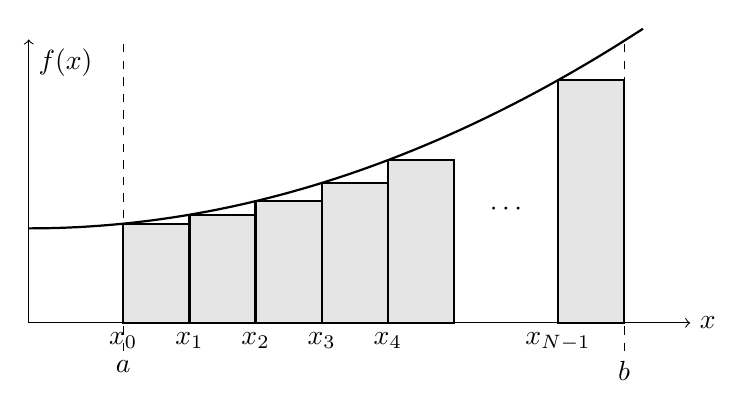
\begin{tikzpicture}[scale=1.2]
  \draw[->] (0,0) -- (7,0) node[right] {$x$};
  \draw[->] (0,0) -- (0,3) node[below right] {$f(x)$};

  \draw[thick, domain=0:6.5, smooth, variable=\x] plot ({\x}, {0.05*\x^2 + 1});

  \node[below] at (1,-0.3) {$a$};
  \draw[dashed] (1,-0.3) -- (1,3);
  \node[below] at (6.3,-0.3) {$b$};
  \draw[dashed] (6.3,-0.3) -- (6.3,3);

  \def\dx{0.7}
  \foreach \i in {0,1,2,3,4} {
    \pgfmathsetmacro{\xleft}{1 + \i*\dx}
    \pgfmathsetmacro{\height}{0.05*\xleft^2 + 1}
    \fill[gray!20] (\xleft,0) rectangle ({\xleft+\dx}, {\height});
    \draw[thick] (\xleft,0) rectangle ({\xleft+\dx}, {\height});
    \node[below] at (\xleft,0) {$x_\i$};
  }

  \node at (5.05,1.2) {$\cdots$};

  \pgfmathsetmacro{\xfinal}{5.6}
  \pgfmathsetmacro{\hfinal}{0.05*\xfinal^2 + 1}
  \node[below] at (\xfinal,0) {$x_{N-1}$};
  \fill[gray!20] (\xfinal,0) rectangle ({\xfinal+\dx}, {\hfinal});
  \draw[thick] (\xfinal,0) rectangle ({\xfinal+\dx}, {\hfinal});
\end{tikzpicture}
\end{center}

\begin{definition}[Riemann Integrable]
  A function $f(x)$ is \textit{Riemann integrable} if the generalised Riemann sum \textbf{does not} depend on how exactly we choose the rectangles in the limit provided all $\Delta x \to 0$ in the limit.

  For example we could have non-uniform $\Delta x$ or evaluate $f$ at the centre or right of each interval.
\end{definition}
To show how this is related to the area under a curve consider a single interval:
\begin{center}
 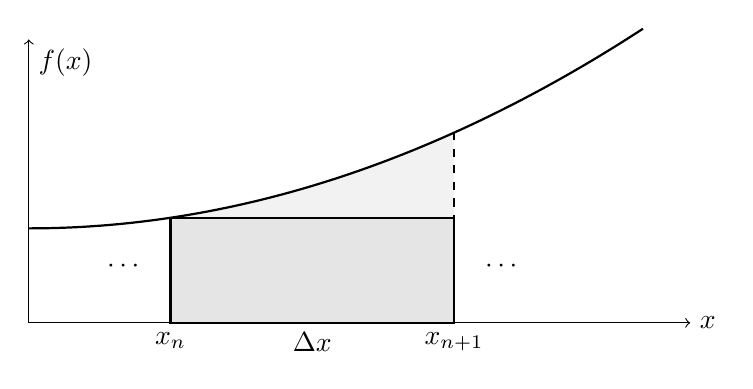
\begin{tikzpicture}[scale=1.2]
  \draw[->] (0,0) -- (7,0) node[right] {$x$};
  \draw[->] (0,0) -- (0,3) node[below right] {$f(x)$};

  \fill [gray!10, domain=1.5:4.5, variable=\x]
    (1.5, 0)
    -- plot ({\x}, {0.05*\x^2 + 1})
    -- (4.5, 0)
    -- cycle;
  \draw[thick, domain=0:6.5, smooth, variable=\x] plot ({\x}, {0.05*\x^2 + 1});

  \pgfmathsetmacro{\height}{0.05*1.5^2 + 1}
  \fill[gray!20] (1.5,0) rectangle (4.5, {\height});
  \draw[thick] (1.5,0) rectangle (4.5, {\height});
  \node at (5,0.6) {$\cdots$};
  \node at (1,0.6) {$\cdots$};
  \node[below] at (1.5,0) {$x_n$};
  \node[below] at (3, 0) {$\Delta x$};
  \node[below] at (4.5,0) {$x_{n+1}$};
  \draw[dashed] (4.5,0) -- (4.5,0.05*4.5^2 + 1);
\end{tikzpicture}
\end{center}
\begin{theorem}[Mean Value Theorem]
  For $f(x)$ continuous, the area under the \textbf{curve} from $x_n$ to $x_{n + 1}$ is:
  \[
    A_n = (x_{n+1}-x_n)f(c_n) = \Delta x f(c_n)
    \label{meanValue}
  \]
  for some $c_n$ with $x_n \leq c_n \leq x_{n+1}$.
\end{theorem}
If $f(x)$ is differentiable, we can use the stronger case of \cref{taylorsThm} to write:
\begin{align*}
  f(c_n) &= f(x_n) + O(c_n - x_n) \quad \text{ as } c_n - x_n \to 0 \\
         &= f(x_n) + O(\Delta x) \text{ since $\Delta x \geq c_n - x_n$}
\end{align*}
So we have that:
\[
  A_n = \Delta x f(x_n) + O((\Delta x)^2) \quad \text{ as } \Delta x \to 0
\]
Therefore the total area from $x=a$ to $x=b$ is:
\begin{align*}
  A &= \lim_{N \to \infty} \sum_{n=0}^{N-1} A_n \\
    &= \lim_{N \to \infty} \sum_{n=0}^{N-1} f(x_n) \Delta x + \lim_{N \to \infty} \underbrace{NO\left[\left(\frac{b-a}{N}\right)^2\right]}_{O(1/N)} \\
    &= \int_{a}^{b} f(x) \d{x} + 0
\end{align*}
\subsection{Fundamental Theorem of Calculus}
\begin{theorem}[Fundemental Theorem of Calculus]
  If
  \[
    F(x) = \int_{a}^{x} f(t) \d{t}
  \]
  then:
  \[
    \deriv{F}{x} = \deriv{}{x}\left(\int_{a}^{x} f(t) \d{t}\right) = f(x)
  \]
\end{theorem}
\begin{proof}
  \begin{align*}
    \deriv{F}{x} &= \lim_{h \to 0} \frac{1}{h} \left[\int_{a}^{x+h} f(t) \d{t} - \int_{a}^{x} f(t) \d{t}\right] \\
                 &= \lim_{h \to 0} \frac{1}{h} \left[\int_{x}^{x+h} f(t) \d{t}\right] \\
                 &= \lim_{h \to 0} \frac{1}{h} \left[hf(c)\right] \text{ with } x \leq c \leq x + h \text{ from \cref{meanValue}} \\
                 &= \lim_{h \to 0} [f(x) + O(c-x)] \text{ from \cref{taylorsThm}} \\
                 &=\lim_{h \to 0} [f(x) + O(h)] \text{ since $h \geq c-x$} \\
                 &= f(x)
  \end{align*}
\end{proof}
\begin{remark}[Note]
  $F(x)$ is a solution to the differential equation:
  \[
    \deriv{F}{x} = f(x) \text{ with } F(a) = 0
  \]
\end{remark}
\begin{corollary}
  We can swap the limits for:
  \[
    \deriv{}{x}\left(\int_{x}^{b} f(t) \d{t}\right) = -f(x)
  \]
  We can use the chain rule to get:
  \begin{align*}
    \deriv{}{x}\left(\int_{a}^{g(x)} f(t) \d{t}\right) &= \deriv{}{x}F(g(x)) \\
                                            &= \deriv{F}{g} \deriv{g}{x} \\
                                            &= f(g(x)) g'(x)
  \end{align*}
\end{corollary}
\begin{remark}[Notation]
  We denote indefinite integrals as:
  \[
    \int f(x) \d{x} \text{ or } \int_{}^{x} f(x) \d{x}
  \]
  In the latter case, the unspecified lower limit gives rise to the integration constant.
\end{remark}
\subsection{Integration Techniques}
\subsubsection{Substitution}
If the integrand contains a function of another function, it might help to substitute for the inner function.
\begin{example}
  Consider:
  \[
    I = \int \frac{1-2x}{\sqrt{x - x^2}} \d{x}
  \]
  Let $u = x - x^2$ so $\deriv{u}{x} = 1 - 2x$.
  So
  \[
    I = \int \frac{\d{u}}{\sqrt{u}} = 2\sqrt{u} + C = 2\sqrt{x - x^2} + C
  \]
\end{example}
\subsubsection{Trig. Substitutions}
\begin{center}
\begin{tabular}{c|c|c}
Identity & Integrand Contains & Subtitution \\
\hline
$\cos^2 \theta  + \sin^2 \theta = 1$ & $\sqrt{1-x^2}$ & $x = \sin\theta$ \\
$1 + \tan^2 \theta = \sec^2 \theta$ & $1 + x^2$ & $x = \tan \theta$ \\
$\cosh^2u - \sinh^2u = 1$ & $\sqrt{x^2 + 1}$ & $x = \sinh u$ \\
$\cosh^2u - \sinh^2u = 1$ & $\sqrt{x^2 - 1}$ & $x = \cosh u$ \\
$1-\tanh^2u = \sech^2u$ & $1-x^2$ & $x = \tanh u$
\end{tabular}
\end{center}
\begin{example}
  Consider:
  \[
    I = \int \sqrt{2x - x^2} \d{x} = \int \sqrt{1 - (x-1)^2} \d{x} \\
  \]
  Try $x - 1 = \sin \theta$ so $\d{x} = \cos\theta \d{\theta}$ with $-\pi/2 \leq \theta \leq \pi/2$ which is unique for $0 \leq x \leq 2$.
  \begin{align*}
    I &= \int \sqrt{\cos^2\theta} \d{\theta} \\
      &= \int \cos^2 \theta \d{x} \\
      &= \frac{1}{2} \int 1 + \cos 2\theta \d{x} \\
      &= \frac{1}{2}(\theta + \sin\theta \cos \theta) + C \\
      &= \frac{1}{2} \arcsin(x-1) + \frac{1}{2}(x-1)\sqrt{1 - (x-1)^2} + C
  \end{align*}
\end{example}
\end{document}
